\documentclass{article}
\usepackage{tabularx}
\usepackage{longtable}
\usepackage{array}
\usepackage{float}
\usepackage{listings}
\usepackage{amsmath}
\usepackage{amssymb}
\usepackage{mathtools}
\usepackage{amsfonts}
\usepackage{graphicx}
\usepackage[table]{xcolor}
\setlength{\arrayrulewidth}{0.5mm}
\graphicspath{ {./images/} }
\usepackage[margin=20mm]{geometry}
\renewcommand{\labelenumii}{\theenumii}
\renewcommand{\theenumii}{\theenumi.\arabic{enumii}.}
\renewcommand{\arraystretch}{1.5}
\newcommand{\f}[2]{f_{#1}(#2)}
\newcommand{\code}[1]{\texttt{#1}}
\DeclarePairedDelimiter{\ceil}{\lceil}{\rceil}
\DeclarePairedDelimiter{\set}{\left\{}{\right\}}
\DeclarePairedDelimiter{\parens}{\lparen}{\rparen}
\title{HW3 Report}
\date{}
\begin{document}
\maketitle
\section*{Section 1}
\subsection*{Q1:}
    \begin{figure}[H]
        \centering
        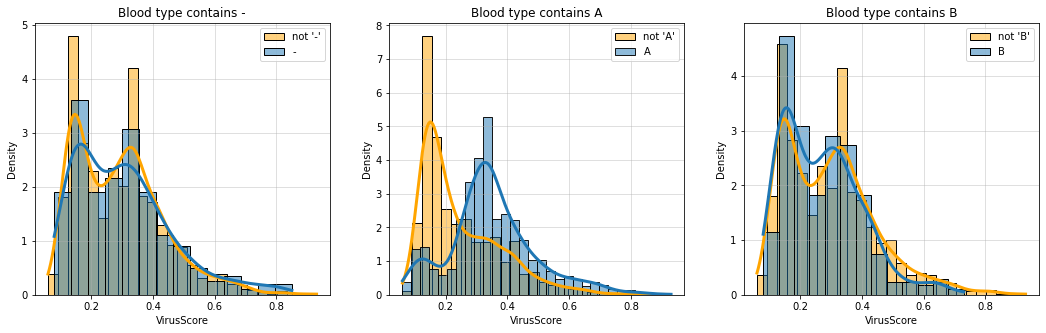
\includegraphics[scale=0.5]{images/q1.png}
        \caption{KDE plots of \code{VirusScore} conditioned different conditions of \code{blood\_type}}
        \label{fig:q1}
    \end{figure}
\subsection*{Q2:}
    \paragraph*{}
    In figure \ref{fig:q1} in the plot of A versus not A, we observe that the groups of patients with and and without "A" in their blood types are mostly seperable along a boundary that is approximately the \code{VirusScore} of $0.225$. 
    \paragraph*{}
    Therefore, the condition of contains/does not contain A would be most informative for learning \code{VirusScore}.
    As it turns out, we decided already in hw1 to create this feature.
\subsection*{Q3:}
    \begin{figure}[H]
        \centering
        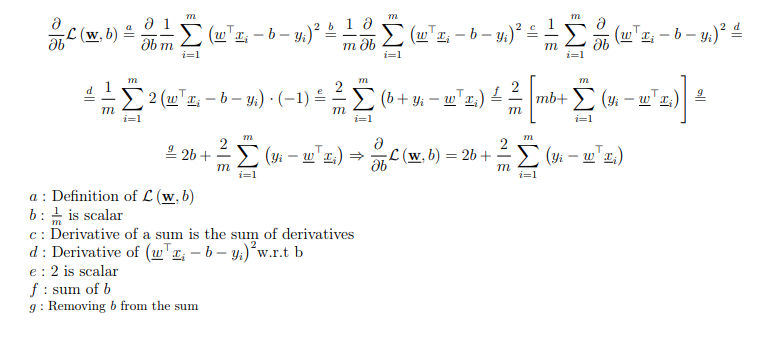
\includegraphics[scale=0.7]{images/q3.png}
    \end{figure}

\end{document}